\documentclass[]{article}
\usepackage{lmodern}
\usepackage{amssymb,amsmath}
\usepackage{ifxetex,ifluatex}
\usepackage{fixltx2e} % provides \textsubscript
\ifnum 0\ifxetex 1\fi\ifluatex 1\fi=0 % if pdftex
  \usepackage[T1]{fontenc}
  \usepackage[utf8]{inputenc}
\else % if luatex or xelatex
  \ifxetex
    \usepackage{mathspec}
  \else
    \usepackage{fontspec}
  \fi
  \defaultfontfeatures{Ligatures=TeX,Scale=MatchLowercase}
\fi
% use upquote if available, for straight quotes in verbatim environments
\IfFileExists{upquote.sty}{\usepackage{upquote}}{}
% use microtype if available
\IfFileExists{microtype.sty}{%
\usepackage{microtype}
\UseMicrotypeSet[protrusion]{basicmath} % disable protrusion for tt fonts
}{}
\usepackage[margin=1in]{geometry}
\usepackage{hyperref}
\hypersetup{unicode=true,
            pdftitle={Chapter Four},
            pdfauthor={Ryan Honea},
            pdfborder={0 0 0},
            breaklinks=true}
\urlstyle{same}  % don't use monospace font for urls
\usepackage{color}
\usepackage{fancyvrb}
\newcommand{\VerbBar}{|}
\newcommand{\VERB}{\Verb[commandchars=\\\{\}]}
\DefineVerbatimEnvironment{Highlighting}{Verbatim}{commandchars=\\\{\}}
% Add ',fontsize=\small' for more characters per line
\usepackage{framed}
\definecolor{shadecolor}{RGB}{248,248,248}
\newenvironment{Shaded}{\begin{snugshade}}{\end{snugshade}}
\newcommand{\KeywordTok}[1]{\textcolor[rgb]{0.13,0.29,0.53}{\textbf{{#1}}}}
\newcommand{\DataTypeTok}[1]{\textcolor[rgb]{0.13,0.29,0.53}{{#1}}}
\newcommand{\DecValTok}[1]{\textcolor[rgb]{0.00,0.00,0.81}{{#1}}}
\newcommand{\BaseNTok}[1]{\textcolor[rgb]{0.00,0.00,0.81}{{#1}}}
\newcommand{\FloatTok}[1]{\textcolor[rgb]{0.00,0.00,0.81}{{#1}}}
\newcommand{\ConstantTok}[1]{\textcolor[rgb]{0.00,0.00,0.00}{{#1}}}
\newcommand{\CharTok}[1]{\textcolor[rgb]{0.31,0.60,0.02}{{#1}}}
\newcommand{\SpecialCharTok}[1]{\textcolor[rgb]{0.00,0.00,0.00}{{#1}}}
\newcommand{\StringTok}[1]{\textcolor[rgb]{0.31,0.60,0.02}{{#1}}}
\newcommand{\VerbatimStringTok}[1]{\textcolor[rgb]{0.31,0.60,0.02}{{#1}}}
\newcommand{\SpecialStringTok}[1]{\textcolor[rgb]{0.31,0.60,0.02}{{#1}}}
\newcommand{\ImportTok}[1]{{#1}}
\newcommand{\CommentTok}[1]{\textcolor[rgb]{0.56,0.35,0.01}{\textit{{#1}}}}
\newcommand{\DocumentationTok}[1]{\textcolor[rgb]{0.56,0.35,0.01}{\textbf{\textit{{#1}}}}}
\newcommand{\AnnotationTok}[1]{\textcolor[rgb]{0.56,0.35,0.01}{\textbf{\textit{{#1}}}}}
\newcommand{\CommentVarTok}[1]{\textcolor[rgb]{0.56,0.35,0.01}{\textbf{\textit{{#1}}}}}
\newcommand{\OtherTok}[1]{\textcolor[rgb]{0.56,0.35,0.01}{{#1}}}
\newcommand{\FunctionTok}[1]{\textcolor[rgb]{0.00,0.00,0.00}{{#1}}}
\newcommand{\VariableTok}[1]{\textcolor[rgb]{0.00,0.00,0.00}{{#1}}}
\newcommand{\ControlFlowTok}[1]{\textcolor[rgb]{0.13,0.29,0.53}{\textbf{{#1}}}}
\newcommand{\OperatorTok}[1]{\textcolor[rgb]{0.81,0.36,0.00}{\textbf{{#1}}}}
\newcommand{\BuiltInTok}[1]{{#1}}
\newcommand{\ExtensionTok}[1]{{#1}}
\newcommand{\PreprocessorTok}[1]{\textcolor[rgb]{0.56,0.35,0.01}{\textit{{#1}}}}
\newcommand{\AttributeTok}[1]{\textcolor[rgb]{0.77,0.63,0.00}{{#1}}}
\newcommand{\RegionMarkerTok}[1]{{#1}}
\newcommand{\InformationTok}[1]{\textcolor[rgb]{0.56,0.35,0.01}{\textbf{\textit{{#1}}}}}
\newcommand{\WarningTok}[1]{\textcolor[rgb]{0.56,0.35,0.01}{\textbf{\textit{{#1}}}}}
\newcommand{\AlertTok}[1]{\textcolor[rgb]{0.94,0.16,0.16}{{#1}}}
\newcommand{\ErrorTok}[1]{\textcolor[rgb]{0.64,0.00,0.00}{\textbf{{#1}}}}
\newcommand{\NormalTok}[1]{{#1}}
\usepackage{longtable,booktabs}
\usepackage{graphicx,grffile}
\makeatletter
\def\maxwidth{\ifdim\Gin@nat@width>\linewidth\linewidth\else\Gin@nat@width\fi}
\def\maxheight{\ifdim\Gin@nat@height>\textheight\textheight\else\Gin@nat@height\fi}
\makeatother
% Scale images if necessary, so that they will not overflow the page
% margins by default, and it is still possible to overwrite the defaults
% using explicit options in \includegraphics[width, height, ...]{}
\setkeys{Gin}{width=\maxwidth,height=\maxheight,keepaspectratio}
\IfFileExists{parskip.sty}{%
\usepackage{parskip}
}{% else
\setlength{\parindent}{0pt}
\setlength{\parskip}{6pt plus 2pt minus 1pt}
}
\setlength{\emergencystretch}{3em}  % prevent overfull lines
\providecommand{\tightlist}{%
  \setlength{\itemsep}{0pt}\setlength{\parskip}{0pt}}
\setcounter{secnumdepth}{0}
% Redefines (sub)paragraphs to behave more like sections
\ifx\paragraph\undefined\else
\let\oldparagraph\paragraph
\renewcommand{\paragraph}[1]{\oldparagraph{#1}\mbox{}}
\fi
\ifx\subparagraph\undefined\else
\let\oldsubparagraph\subparagraph
\renewcommand{\subparagraph}[1]{\oldsubparagraph{#1}\mbox{}}
\fi

%%% Use protect on footnotes to avoid problems with footnotes in titles
\let\rmarkdownfootnote\footnote%
\def\footnote{\protect\rmarkdownfootnote}

%%% Change title format to be more compact
\usepackage{titling}

% Create subtitle command for use in maketitle
\newcommand{\subtitle}[1]{
  \posttitle{
    \begin{center}\large#1\end{center}
    }
}

\setlength{\droptitle}{-2em}
  \title{Chapter Four}
  \pretitle{\vspace{\droptitle}\centering\huge}
  \posttitle{\par}
  \author{Ryan Honea}
  \preauthor{\centering\large\emph}
  \postauthor{\par}
  \date{}
  \predate{}\postdate{}

\usepackage{bbm}
\usepackage{bm}

\begin{document}
\maketitle

\subsection{Exercise One}\label{exercise-one}

\paragraph{Question}\label{question}

The data in Table the table below show the numbers of cases of AIDS in
Australia by date of diagnosis for successive 3-months periods from 1984
to 1988. (Data from National Centre for HIV Epidemiology and Clinical
Research 1994.)

In this early phase of the epidemic, the numbers of cases seemed to be
increasing exponentially.

\begin{center}
\begin{tabular}{@{}crrrr@{}}
\toprule
     & \multicolumn{4}{c}{Quarter} \\
Year & 1     & 2     & 3    & 4    \\ \midrule
1984 & 1     & 6     & 16   & 23   \\
1985 & 27    & 39    & 31   & 30   \\
1986 & 43    & 51    & 63   & 70   \\
1987 & 88    & 97    & 91   & 104  \\
1988 & 110   & 113   & 149  & 159  \\ \bottomrule
\end{tabular}
\end{center}

\paragraph{Solutions}\label{solutions}

\textbf{(a)}: Plot the number of cases \(y_i\) against time period \(i\)
(\(i = 1,...,20\)).

\emph{Solution: }

\begin{Shaded}
\begin{Highlighting}[]
\NormalTok{time <-}\StringTok{ }\KeywordTok{seq}\NormalTok{(}\DecValTok{1}\NormalTok{,}\DecValTok{20}\NormalTok{,}\DataTypeTok{by=}\DecValTok{1}\NormalTok{)}
\NormalTok{cases <-}\StringTok{ }\KeywordTok{c}\NormalTok{(}\DecValTok{01}\NormalTok{, }\DecValTok{06}\NormalTok{, }\DecValTok{16}\NormalTok{, }\DecValTok{23}\NormalTok{, }\DecValTok{27}\NormalTok{, }\DecValTok{039}\NormalTok{, }\DecValTok{031}\NormalTok{, }\DecValTok{030}\NormalTok{, }\DecValTok{043}\NormalTok{, }\DecValTok{051}\NormalTok{,}
          \DecValTok{63}\NormalTok{, }\DecValTok{70}\NormalTok{, }\DecValTok{88}\NormalTok{, }\DecValTok{97}\NormalTok{, }\DecValTok{91}\NormalTok{, }\DecValTok{104}\NormalTok{, }\DecValTok{110}\NormalTok{, }\DecValTok{113}\NormalTok{, }\DecValTok{149}\NormalTok{, }\DecValTok{159}\NormalTok{)}
\KeywordTok{plot}\NormalTok{(cases ~}\StringTok{ }\NormalTok{time)}
\end{Highlighting}
\end{Shaded}

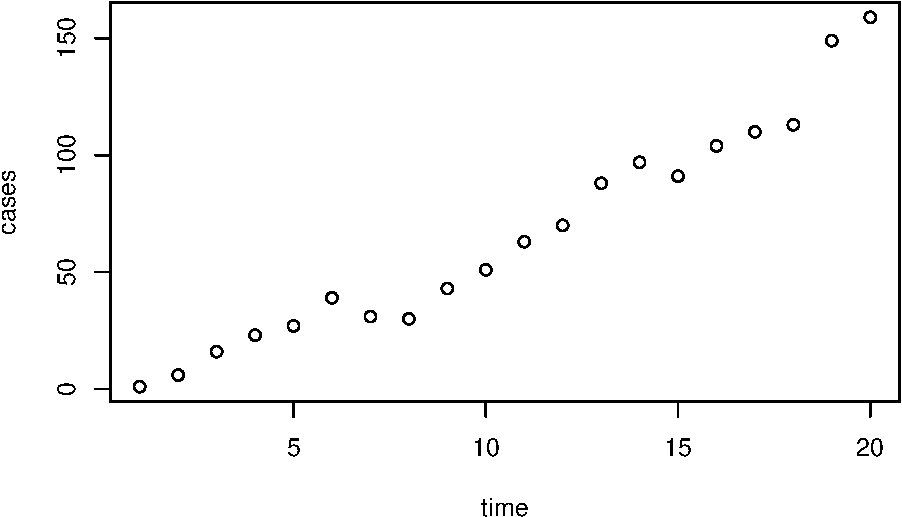
\includegraphics{ExercisesWithSolutions_files/figure-latex/unnamed-chunk-1-1.pdf}

\textbf{(b)}: A possible model is the Poisson distribution with
parameter \(\lambda_i = i^\theta\), or equivelantly \[
\log\lambda_i = \theta\log i.
\] Plot \(\log y_i\) against \(\log i\) to examine this model.

\emph{Solution: }

\begin{Shaded}
\begin{Highlighting}[]
\NormalTok{log_cases =}\StringTok{ }\KeywordTok{log}\NormalTok{(cases)}
\NormalTok{log_time =}\StringTok{ }\KeywordTok{log}\NormalTok{(time)}
\KeywordTok{plot}\NormalTok{(log_time, log_cases)}
\end{Highlighting}
\end{Shaded}

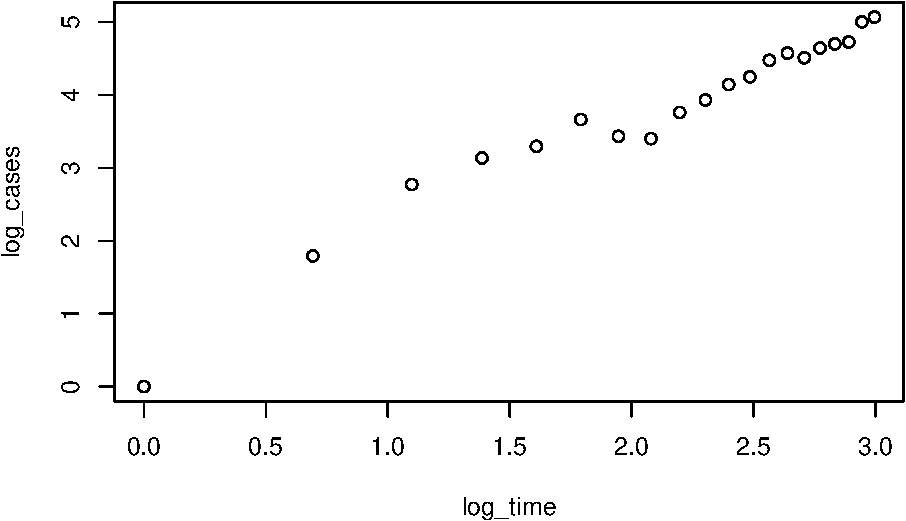
\includegraphics{ExercisesWithSolutions_files/figure-latex/unnamed-chunk-2-1.pdf}

\textbf{(c)}: Fit a generalized linear model to these data using the
Poisson distribution, the log-link function and the equation \[
g(\lambda_i) = \log\lambda_i = \beta_1 + \beta_2x_i,
\] where \(x_i = \log i\). Firstly, do this from first principles,
working out expressions for the weight matrix \(\bm{W}\) and other terms
needed for the iterative equation \[
\bm{X}^T\bm{WXb}^{(m)} = \bm{X}^T\bm{Wz}
\] and using software which can perform matrix operations to carry out
the calculations.

\emph{Solution: } Note that \[
w_{ii} = \frac{1}{\text{var}(Y_i)}\left(\frac{\partial \mu_i}{\partial \eta_i}\right)^2
\] and \[
z_i = \sum_{k=1}^px_{ik}b_k^{(m-1)} + (y_i - \mu_i)\left(\frac{\partial \eta_i}{\partial \mu_i}\right)
\]

and these are the values for which we must find solutions.

In this case,
\(\mu_i = \lambda_i = e^{\beta_1 + \beta_2x_i} = e^{\eta_i}\) and thus
\(\frac{\partial \mu_i}{\partial \eta_i} = e^{\eta_i}\). We also know
that \(\text{var}(Y_i)\) of a Poisson is just \(\lambda_i\) (where
\(\lambda_i = e^{\eta_i}\) here). Therefore we have \[
w_{ii} = \frac{1}{e^{\eta_i}}\left(e^{\eta_i}\right)^2 = e^{\eta_i} = e^{\bm{x}_i^T\bm{\beta}}.
\] and

\begin{align*}
z_i &= \bm{x}_i\bm{\beta} + (y_i - e^{\eta_i})(e^{\eta_i})\\
    &= \eta_i + (y_i - e^{\eta_i})e^{-\eta_i}\\
    &= \eta_i + \frac{y_i}{\eta_i} - 1
\end{align*}

We can therefore solve this with the following iterative R code
initializing our \(\bm{\beta}\) to the means of the \(x_i\).

\begin{Shaded}
\begin{Highlighting}[]
\KeywordTok{require}\NormalTok{(MASS)}
\end{Highlighting}
\end{Shaded}

\begin{verbatim}
## Loading required package: MASS
\end{verbatim}

\begin{Shaded}
\begin{Highlighting}[]
\NormalTok{x =}\StringTok{ }\KeywordTok{as.matrix}\NormalTok{(}\KeywordTok{log}\NormalTok{(time))}
\NormalTok{y =}\StringTok{ }\KeywordTok{as.matrix}\NormalTok{(cases)}
\NormalTok{x =}\StringTok{ }\KeywordTok{cbind}\NormalTok{(}\KeywordTok{rep}\NormalTok{(}\DecValTok{1}\NormalTok{,}\KeywordTok{length}\NormalTok{(x)), x)}
\NormalTok{b =}\StringTok{ }\KeywordTok{as.matrix}\NormalTok{(}\KeywordTok{c}\NormalTok{(}\KeywordTok{mean}\NormalTok{(x[,}\DecValTok{1}\NormalTok{]),}\KeywordTok{mean}\NormalTok{(x[,}\DecValTok{2}\NormalTok{])))}
\NormalTok{for (i in }\DecValTok{1}\NormalTok{:}\DecValTok{1000}\NormalTok{) \{}
  \NormalTok{oldb =}\StringTok{ }\NormalTok{b}
  \NormalTok{w_ii =}\StringTok{ }\KeywordTok{exp}\NormalTok{(x%*%b)}
  \NormalTok{W =}\StringTok{ }\KeywordTok{diag}\NormalTok{(w_ii[,])}
  \NormalTok{z =}\StringTok{ }\NormalTok{x %*%}\StringTok{ }\NormalTok{b +}\StringTok{ }\NormalTok{y/}\KeywordTok{exp}\NormalTok{(x%*%b) -}\StringTok{ }\DecValTok{1}
  \NormalTok{b =}\StringTok{ }\KeywordTok{solve}\NormalTok{(}\KeywordTok{t}\NormalTok{(x) %*%}\StringTok{ }\NormalTok{W %*%}\StringTok{ }\NormalTok{x) %*%}\StringTok{ }\NormalTok{(}\KeywordTok{t}\NormalTok{(x) %*%}\StringTok{ }\NormalTok{W %*%}\StringTok{ }\NormalTok{z)}
  \NormalTok{b1 =}\StringTok{ }\KeywordTok{sprintf}\NormalTok{(}\StringTok{"%.5f"}\NormalTok{, b[}\DecValTok{1}\NormalTok{])}
  \NormalTok{b2 =}\StringTok{ }\KeywordTok{sprintf}\NormalTok{(}\StringTok{"%.5f"}\NormalTok{, b[}\DecValTok{2}\NormalTok{])}
  \KeywordTok{cat}\NormalTok{(}\StringTok{"Iteration"}\NormalTok{, i, }\StringTok{": b1 = "}\NormalTok{, b1, }\StringTok{", b2 = "}\NormalTok{, b2, }\StringTok{"}\CharTok{\textbackslash{}n}\StringTok{"}\NormalTok{)}
  \NormalTok{if (}\KeywordTok{abs}\NormalTok{(oldb[}\DecValTok{1}\NormalTok{] -}\StringTok{ }\NormalTok{b[}\DecValTok{1}\NormalTok{]) <}\StringTok{ }\NormalTok{.}\DecValTok{0005} \NormalTok{&}\StringTok{ }\KeywordTok{abs}\NormalTok{(oldb[}\DecValTok{2}\NormalTok{] -}\StringTok{ }\NormalTok{b[}\DecValTok{2}\NormalTok{]) <}\StringTok{ }\NormalTok{.}\DecValTok{0005}\NormalTok{) \{}
    \KeywordTok{cat}\NormalTok{(}\StringTok{"Converged at"}\NormalTok{, i, }\StringTok{"iterations"}\NormalTok{)}
    \NormalTok{break}
  \NormalTok{\}}
\NormalTok{\}}
\end{Highlighting}
\end{Shaded}

\begin{verbatim}
## Iteration 1 : b1 =  0.47222 , b2 =  1.98729 
## Iteration 2 : b1 =  0.43624 , b2 =  1.73805 
## Iteration 3 : b1 =  0.79247 , b2 =  1.45112 
## Iteration 4 : b1 =  0.98230 , b2 =  1.33503 
## Iteration 5 : b1 =  0.99594 , b2 =  1.32665 
## Iteration 6 : b1 =  0.99600 , b2 =  1.32661 
## Converged at 6 iterations
\end{verbatim}

\textbf{(d)}: Fit the model in (c) using statistical software which can
perform Poisson regression. Compare the results with those obtained in
(c).

\begin{Shaded}
\begin{Highlighting}[]
\NormalTok{glmod <-}\StringTok{ }\KeywordTok{glm}\NormalTok{(cases ~}\StringTok{ }\KeywordTok{log}\NormalTok{(time), }\DataTypeTok{family =} \StringTok{"poisson"}\NormalTok{)}
\KeywordTok{cat}\NormalTok{(}\StringTok{"b1 ="}\NormalTok{, glmod$coefficients[}\DecValTok{1}\NormalTok{], }\StringTok{"}\CharTok{\textbackslash{}n}\StringTok{b2 ="}\NormalTok{, glmod$coefficients[}\DecValTok{2}\NormalTok{])}
\end{Highlighting}
\end{Shaded}

\begin{verbatim}
## b1 = 0.995998 
## b2 = 1.32661
\end{verbatim}

The results of the model using the built in \texttt{glm} feature in R
are the same as the results from the code in part \textbf{c}.

\pagebreak

\subsection{Exercise Two}\label{exercise-two}

\paragraph{Question}\label{question-1}

The data in the table below are times to death, \(y_i\), in weeks from
diagnosis and \(\log_{10}\)(initial white blood cell count), \(x_i\),
for seventeen patients suffering from leukemia. (This is Example U from
Cox and Snell 1981.)

\begin{center}
\begin{tabular}{@{}crrrrrrrrr@{}}
\toprule
$y_i$ & 65   & 156  & 100  & 134  & 16   & 108  & 121  & 4    & 39   \\
$x_i$ & 3.36 & 2.88 & 3.63 & 3.41 & 3.78 & 4.02 & 4.00 & 4.23 & 3.73 \\
      &      &      &      &      &      &      &      &      &      \\
$y_i$ & 143  & 56   & 26   & 22   & 1    & 1    & 5    & 65   &      \\
$x_i$ & 3.85 & 3.97 & 4.51 & 4.54 & 5.00 & 5.00 & 4.72 & 5.00 &      \\ \bottomrule
\end{tabular}
\end{center}

\paragraph{Solutions}\label{solutions-1}

\textbf{(a)}: Plot \(y_i\) against \(x_i\). Do the data show any trends?

\emph{Solution: }

\begin{Shaded}
\begin{Highlighting}[]
\NormalTok{x <-}\StringTok{ }\KeywordTok{c}\NormalTok{(}\FloatTok{3.36}\NormalTok{, }\FloatTok{2.88}\NormalTok{, }\FloatTok{3.63}\NormalTok{, }\FloatTok{3.41}\NormalTok{, }\FloatTok{3.78}\NormalTok{, }\FloatTok{4.02}\NormalTok{, }\FloatTok{4.00}\NormalTok{, }\FloatTok{4.23}\NormalTok{, }\FloatTok{3.73}\NormalTok{,}
       \FloatTok{3.85}\NormalTok{, }\FloatTok{3.97}\NormalTok{, }\FloatTok{4.51}\NormalTok{, }\FloatTok{4.54}\NormalTok{, }\FloatTok{5.00}\NormalTok{, }\FloatTok{5.00}\NormalTok{, }\FloatTok{4.72}\NormalTok{, }\FloatTok{5.00}\NormalTok{)}
\NormalTok{y <-}\StringTok{ }\KeywordTok{c}\NormalTok{(}\DecValTok{065}\NormalTok{, }\DecValTok{156}\NormalTok{, }\DecValTok{100}\NormalTok{, }\DecValTok{134}\NormalTok{, }\DecValTok{016}\NormalTok{, }\DecValTok{108}\NormalTok{, }\DecValTok{121}\NormalTok{, }\DecValTok{004}\NormalTok{, }\DecValTok{039}\NormalTok{,}
       \DecValTok{143}\NormalTok{, }\DecValTok{056}\NormalTok{, }\DecValTok{026}\NormalTok{, }\DecValTok{022}\NormalTok{, }\DecValTok{001}\NormalTok{, }\DecValTok{001}\NormalTok{, }\DecValTok{005}\NormalTok{, }\DecValTok{065}\NormalTok{)}
\NormalTok{df <-}\StringTok{ }\KeywordTok{data.frame}\NormalTok{(}\KeywordTok{cbind}\NormalTok{(x, y))}
\KeywordTok{plot}\NormalTok{(df$x, df$y)}
\KeywordTok{abline}\NormalTok{(}\KeywordTok{lm}\NormalTok{(df$y ~}\StringTok{ }\NormalTok{df$x))}
\end{Highlighting}
\end{Shaded}

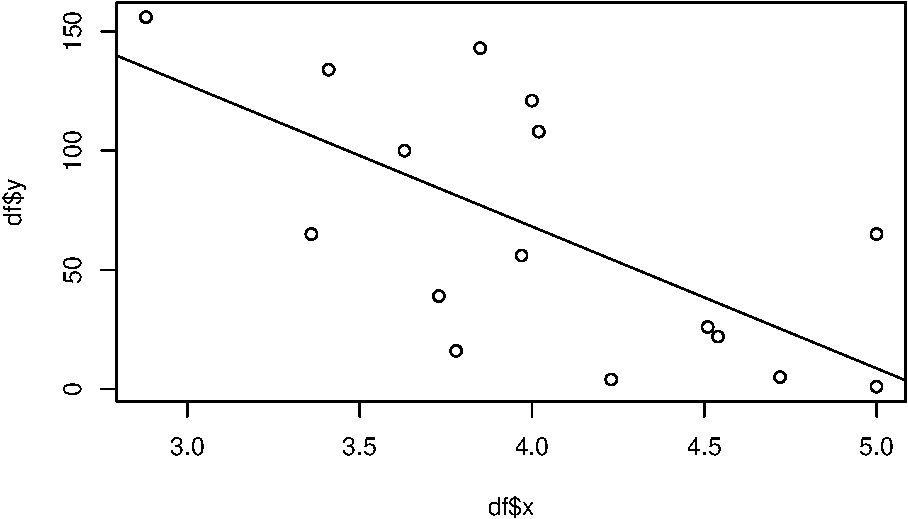
\includegraphics{ExercisesWithSolutions_files/figure-latex/unnamed-chunk-5-1.pdf}

I decided to go ahead and add the line that would come from a typical
linear regression. The only clear trend seems to be a slightly downward
trend, but overall the data seems to be pretty dispersed as it stands
right now.

\textbf{(b)}: A possible specification for \(E(Y)\) is \[
\text{E}(Y_i) = \exp(\beta_1 + \beta_2x_i),
\] which can ensure all E\((Y)\) is non-negative for all values of the
paramaters and all values of \(x\). Which link function is appropriate
in this case?

\begin{Shaded}
\begin{Highlighting}[]
\KeywordTok{plot}\NormalTok{(x, }\KeywordTok{log}\NormalTok{(y))}
\end{Highlighting}
\end{Shaded}

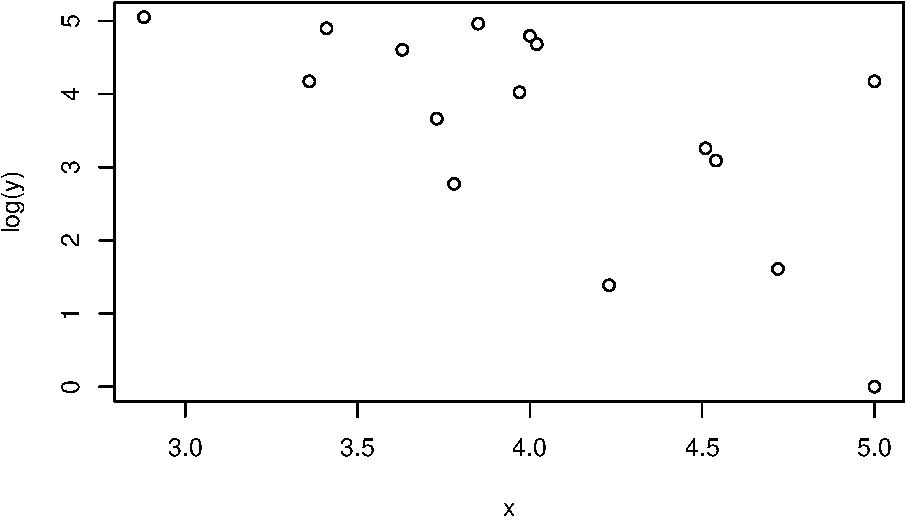
\includegraphics{ExercisesWithSolutions_files/figure-latex/unnamed-chunk-6-1.pdf}

This kind of helps in visualizing a potential model to describe our
results. Again, it seems that the log-link might be our best result.

\textbf{(c)}: The Exponential distribution is often used to describe
survival times. The probability distribution is
\(f(y; \theta) = \theta e^{-y\theta}\). This is a special case of the
Gamma distribution with shape parameters \(\phi = 1\) (see Exercise
3.12(a)). Show that E\((Y) = 1/\theta\) and var\((Y) = 1/\theta^2\).

\emph{Solution: } In Exercise 3.12(a), it was shown that the Exponential
is a special case of the Gamma distribution where \(\alpha = 1\), and
\(\beta = \theta\). The expected value and mean of the gamma
distribution are \(\text{E}[Y] = \frac{\alpha}{\theta}\) and
\(\text{var}[Y] = \frac{\alpha}{\beta^2}\). Therfore,
\(\text{E}[Y] = \frac{1}{\theta}\) and
\(\text{var}[Y] = \frac{1}{\theta^2}\).

\textbf{(d)}: Fit a model with the equation for E\((Y_i)\) given in (b)
and the Exponential distribution using appropriate statistical software.

\begin{Shaded}
\begin{Highlighting}[]
\NormalTok{glmod <-}\StringTok{ }\KeywordTok{glm}\NormalTok{(y ~}\StringTok{ }\NormalTok{x, }\DataTypeTok{family =} \KeywordTok{Gamma}\NormalTok{(}\DataTypeTok{link =} \StringTok{"log"}\NormalTok{))}
\KeywordTok{cat}\NormalTok{(}\StringTok{"b1 ="}\NormalTok{, glmod$coefficients[}\DecValTok{1}\NormalTok{], }\StringTok{"}\CharTok{\textbackslash{}n}\StringTok{b2 ="}\NormalTok{, glmod$coefficients[}\DecValTok{2}\NormalTok{])}
\end{Highlighting}
\end{Shaded}

\begin{verbatim}
## b1 = 8.477494 
## b2 = -1.109297
\end{verbatim}

\textbf{(e)}: For the model fitted in (d), compare the observed values
\(y_i\), and fitted values
\(\hat{y_i} = \exp(\hat{\beta_1} + \hat{\beta_2}x_i),\) and use the
standardized residuals \(r_i = (y_i - \hat{y_i})/\hat{y_i}\) to
investigate the adequacy of the model. (Note: \(\hat{y_i}\) is used as
the denominator of \(r_i\) because it is an estimate of the standard
deviation of \(Y_i\)--see (c) above.)

\begin{Shaded}
\begin{Highlighting}[]
\NormalTok{predictions =}\StringTok{ }\KeywordTok{predict}\NormalTok{(glmod, }\KeywordTok{list}\NormalTok{(}\DataTypeTok{x =} \NormalTok{x), }\DataTypeTok{type=} \StringTok{"resp"}\NormalTok{)}
\NormalTok{residuals =}\StringTok{ }\NormalTok{(y -}\StringTok{ }\NormalTok{predictions)/predictions}
\NormalTok{residuals}
\end{Highlighting}
\end{Shaded}

\begin{verbatim}
##           1           2           3           4           5           6 
## -0.43778372 -0.20773747  0.16698607  0.22513214 -0.77947903  0.94256889 
##           7           8           9          10          11          12 
##  1.12864291 -0.90917977 -0.49148188  1.13004731 -0.04708838 -0.19464163 
##          13          14          15          16          17 
## -0.29548320 -0.94665681 -0.94665681 -0.80449595  2.46730734
\end{verbatim}

\begin{Shaded}
\begin{Highlighting}[]
\KeywordTok{plot}\NormalTok{(x,y)}
\KeywordTok{curve}\NormalTok{(}\KeywordTok{predict}\NormalTok{(glmod, }\KeywordTok{list}\NormalTok{(}\DataTypeTok{x =} \NormalTok{x), }\DataTypeTok{type=} \StringTok{"resp"}\NormalTok{), }\DataTypeTok{add=}\OtherTok{TRUE}\NormalTok{)}
\end{Highlighting}
\end{Shaded}

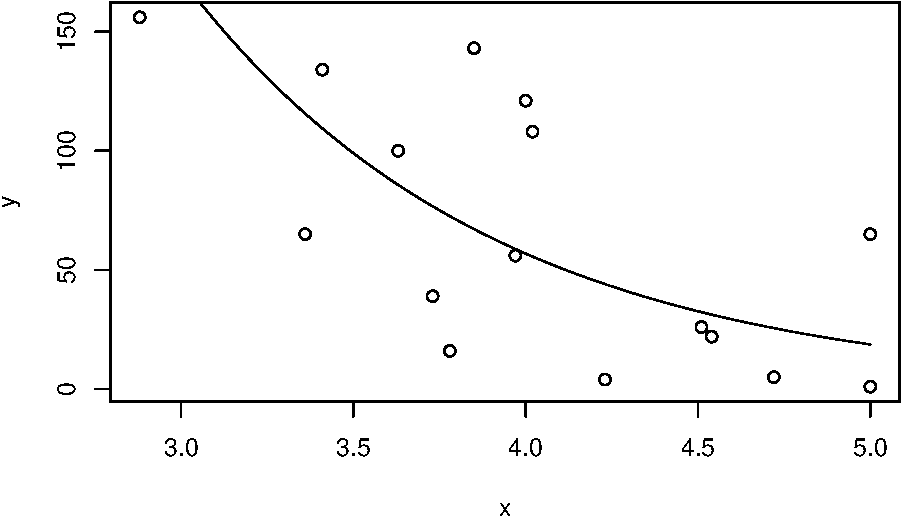
\includegraphics{ExercisesWithSolutions_files/figure-latex/unnamed-chunk-8-1.pdf}

Based on these standardized residuals which are not too far out of
reason, it appears that this fit is actually quite adequate. The plot
seems to show that there are issues, but considering the high variance
of the data, this is perhaps the most adequate fit that is not also in
danger of overfitting.


\end{document}
